\documentclass{report}

% Language setting
% Replace `english' with e.g. `spanish' to change the document language
\usepackage[english]{babel}

% Set page size and margins
% Replace `letterpaper' with `a4paper' for UK/EU standard size
\usepackage[letterpaper,top=2cm,bottom=2cm,left=3cm,right=3cm,marginparwidth=1.75cm]{geometry}

% mdified chapter title to display without "chapter N"
\usepackage{titlesec}
\titleformat{\chapter}[display]
  {\normalfont\bfseries\center}{}{0pt}{\Huge}

% change the name of the abstracts using the  babel package
\addto{\captionsenglish}{\renewcommand{\abstractname}{Executive Summary}}

% place images in place in document
\usepackage{float}

% replaces indentation with blank line
\usepackage[parfill]{parskip}

% ensures no windows and orphans
\usepackage[all]{nowidow}

% insert background images at specific points
\usepackage{wallpaper}

% enumerate with different labels such as alphabetic letter
\usepackage{enumitem}

% Useful packages
\usepackage{amsmath}
\usepackage{graphicx}
\usepackage[colorlinks=true, allcolors=blue]{hyperref}



\begin{document}
% keep outside the begin{document} environment
\begin{titlepage} % Suppresses headers and footers on the title page

	\centering % Centre everything on the title page
	
	\scshape % Use small caps for all text on the title page
	
	\vspace*{\baselineskip} % White space at the top of the page
	
	%------------------------------------------------
	%	Title
	%------------------------------------------------
	
	\rule{\textwidth}{1.6pt}\vspace*{-\baselineskip}\vspace*{2pt} % Thick horizontal rule
	\rule{\textwidth}{0.4pt} % Thin horizontal rule
	
	\vspace{0.75\baselineskip} % Whitespace above the title
	
	{\LARGE NYSC\\ DRUG FREE\\ MANDATE\\} % Title
	
	\vspace{0.75\baselineskip} % Whitespace below the title
	
	\rule{\textwidth}{0.4pt}\vspace*{-\baselineskip}\vspace{3.2pt} % Thin horizontal rule
	\rule{\textwidth}{1.6pt} % Thick horizontal rule
	
	\vspace{2\baselineskip} % Whitespace after the title block
	
	%------------------------------------------------
	%	Subtitle
	%------------------------------------------------
	
% 	A Number of Fascinating and Life-changing Templates Presented in a Clear and Concise Way % Subtitle or further description
	
	\vspace*{3\baselineskip} % Whitespace under the subtitle
	
	%------------------------------------------------
	%	Editor(s)
	%------------------------------------------------
	
	\vspace*{1\baselineskip}
	
	Drafted By
	
	\vspace{0.5\baselineskip} % Whitespace before the editors
	
	{\scshape\Large  Drug Free Club Executives, 2022\\} % Editor list
	\vspace*{3\baselineskip}
	
	Edited By
	
	\vspace{0.5\baselineskip} % Whitespace before the editors
	\vspace*{3\baselineskip}
	\center{........................................................}\\
	{\scshape\Large Victor Ezekiel, General Secretary (2021 C2) \\} % Editor list
	\vspace*{3\baselineskip}
	Approved by
	
	\vspace{0.5\baselineskip} % Whitespace before the editors
	\vspace*{3\baselineskip}
	\center{........................................................}\\
	{\scshape\Large  Ifeoluwa Obisesan, President (2021 B2)\\} % Editor list
	
	\vspace*{3\baselineskip}
	
	Supervised by
	
	\vspace{0.5\baselineskip} % Whitespace before the editors
	\vspace*{3\baselineskip}
	\center{........................................................}\\
	{\scshape\Large  Mr. Habib Tayo, NDLEA NYSC Coordinator (2022)\\} % Editor list
	
	\vspace{0.5\baselineskip} % Whitespace below the editor list
	
	\textit{National Youth Service Commission and National Drug Law Enforcement Agency} % Editor affiliation
	
	\vfill % Whitespace between editor names and publisher logo
	
	%------------------------------------------------
	%	Publisher
	%------------------------------------------------
	
	\plogo % Publisher logo
	
	\vspace{0.3\baselineskip} % Whitespace under the publisher logo
	
	2022 % Publication year
	
	{\large } % Publisher

\end{titlepage}


\begin{abstract}
The Drug Free CDS group is a community development service group within the National Youth Service Corps program setup to provide awareness on the dangers of substance abuse and addiction.
\end{abstract}

\tableofcontents

\chapter{Introduction}
\section{Problem Statement}
The Substance abuse (inclusive of drug abuse) menace globally poses a serious challenge to the society of today and tomorrow. An exponential upsurge has continually been recorded in drug abuse in recurring years, with catalyzing circumstances such as the global pandemic. Reports from 2018, showed 5.5 percent of the global population abuse medical and non-medical drugs, and projections show an additional tens of millions by the year 2030. Particularly challenging is the damning economic and social effects the drug epidemic has wrought with developed countries such as the US reporting over \$100 billion in loss from productivity, crime and destruction attributed to drug abuse.

Developing countries also share in the burden of the epidemic as Africa accounts for 40 \% of global drug abusers. In Nigeria, 14.3 million individuals engaged in drug abuse in 2018 (higher than the global average) and a further 3 million were reported to have a form of abuse disorder ranging from mental and behavioral to physical and sexual disorders. Although, significant policies and agencies (NDLEA, NIDA) have been established to curb the menace and its dangerous efforts on the society, much is still to be done to dampen the rising prevalence of substance abuse and its effects such as intimate partner violence, youth violence, and sexual violence amongst many others. 

Accordingly, due to the vast rural-urban migration, the south-west reports about 22.4 \% of drug abuse victims in the country and states such as Lagos and Ogun reflect high potency of drug and substance abuse. Risk factors ranging from loss of life to torn families and a bleeding society. Youthful (aged 12 - 35) engagement in drug abuse is a challenging facet of the epidemic as schools and parents battle loss of their wards to cultism, internet fraud and violent vices under the influence. Universities report increased student involvements in prostitution and cultism both highly influenced by illegal drug use on campuses.

Conclusively, drug and substance abuse is the only vice common to a 14 year old on the streets of Ota and a 65 year old on Lagos Island. It provides the same concern to a trader and mother as it does to a husband and professional of an abuser. It bears the same self-destructive tendencies to a first-year university student as it does to an elementary student looking to try to improve street toughness. Drug abuse is a destructive menace that needs to be curbed now for a sustainable future tomorrow.

\section{National Youth Service Corps (NYSC)}
The National Youth Service Corps (NYSC) is a program established by the Nigerian government to engage Nigerian graduates in nation building and development. The NYSC scheme was established by Decree No. 24 of 22nd 1973, which has now been repealed and replaced by Decree 51 of 16th June, 1993, with the main goal of "Promoting Unity and Integration Amongst Nigeria Youths." The scheme's primary goal is to instill in Nigerian youths the spirit of selfless service to the nation, as well as to emphasize the spirit of oneness and brotherhood shared by all Nigerians, regardless of cultural background.

The NYSC program is highlighted in four phases (cardinal programs) Orientation, Place of Primary Assignment and Community Development Service. One of the most impacting of this program is the Community Development Service where corps members are expected to identify the various needs of their host communities and mobilize members of their host communities to participate in projects that address those needs creatively.

Like our slogan says, “No to drugs, yes to life!” It’s our innermost desire to see that this menace is eradicated totally from our society, to see that we live in a drug free society for it’s the ideal and healthiest way to live. 

\section{The Drug Free CDS}
The drug free NYSC CDS group is a non-profit group championed by the NDLEA( National Drug Law Enforcement  Agency, founded for the sole purpose of combating the disease, which is drug and substance abuse in the Nigerian society.

\subsection{Drug Free CDS, Ado-Odo Ota Lga, Ogun state, Nigeria.}
The drug free cds group of Ado-Odo Ota local government is a group made up of youths serving in the Ado Odo Ota local government region of Ogun state. It’s a group of concerned youths, determined to effect some changes in the society. Our main aim is to tackle the vice; drug and substance abuse polluting the lives and environment of Ota local government. We want a better future for the youths and the young ones, we seek a violent free environment, a healthier and safer society to live in a society free of hard drugs and substances.

\section{Drug Free Club and the Ota Community}
Looking at this environment in general, it consists of hoodlums that have polluted the environment and a high percentage of drug abuse. It's heartbreaking to see young children getting involved in what the youth are doing. This prevalent attitude has polluted the environment and made it appear unsafe for people. This act has impacted even secondary schools in this community. This demonstrates that the leader has not been fully engaged in these acts.

After much deliberation with the NDLEA, we decided as Drug Free members to impact the community in our own unique way.

\subsection{Activities}
\begin{itemize}
    \item 
    We organize weekly meetings where we extensively enlighten ourselves on drugs and substance abuse. 
    
    \item
    We discuss and deliberate on our goals and how to effectively achieve the said goals. Our other activities include:

\begin{itemize}
    \item 
    Working with the NDLEA to execute projects relating to tackling drug abuse.
    
    \item
    Organize effective sensitization campaigns in schools and the society.
\end{itemize}

\end{itemize}


\section{Mission Statement}
\begin{itemize}
    \item 
    To liberate victims and addicts of substance abuse, reduce the menacing impact of drug abuse and addiction on families and improve the mental well-being of victims by educating members of the public and setting up rehabilitation centers.
    
    \item
    To inspire life-long development in children, youths and young adults (members of the vulnerable population) and prevent effects of drug abuse such as cultism and youth violence by delivering effective sensitization through awareness campaigns and lectures.
\end{itemize}

\section{Vision}
\begin{enumerate}
    \item 
    To educate secondary school students through visits (sensitization) and the placement of a banner as a guideline to follow even when we are no longer in this community.
    
    \item
    To educate the community through various means, such as speaking and having a banner to guide them.
    
    \item
    Create a suggestion application and website on how the community can reach out to us even after we leave this community as Corp members.(remember to remove)
\end{enumerate}

\section{Goals}
The primary goal is to achieve a drug free and safer community, we attain this by firstly, identifying the environmental, biological and behavioral causes of drugs and substance abuse. We wish to bring the following goals to fruition:
\begin{itemize}
    \item 
    Working with the NDLEA to execute projects relating to tackling drug abuse.
    
    \item
    Organize effective sensitization campaigns in schools and the society.
    
    \item
    Conduct about six hours of sensitization per month, touching the lives of 300 pupils, approximately.
    
    \item
    Setting up a functional rehabilitation and recovery center in Sango, Ado-Ota local government, Ogun state, Nigeria.
    
    \item
    Recuperate about 1000 victims of drug abuse annually from the streets.
\end{itemize}


\chapter{Structure of The Drug Free Club}
\section{Organogram OF NYSC}
\begin{figure}[H]
    \centering
    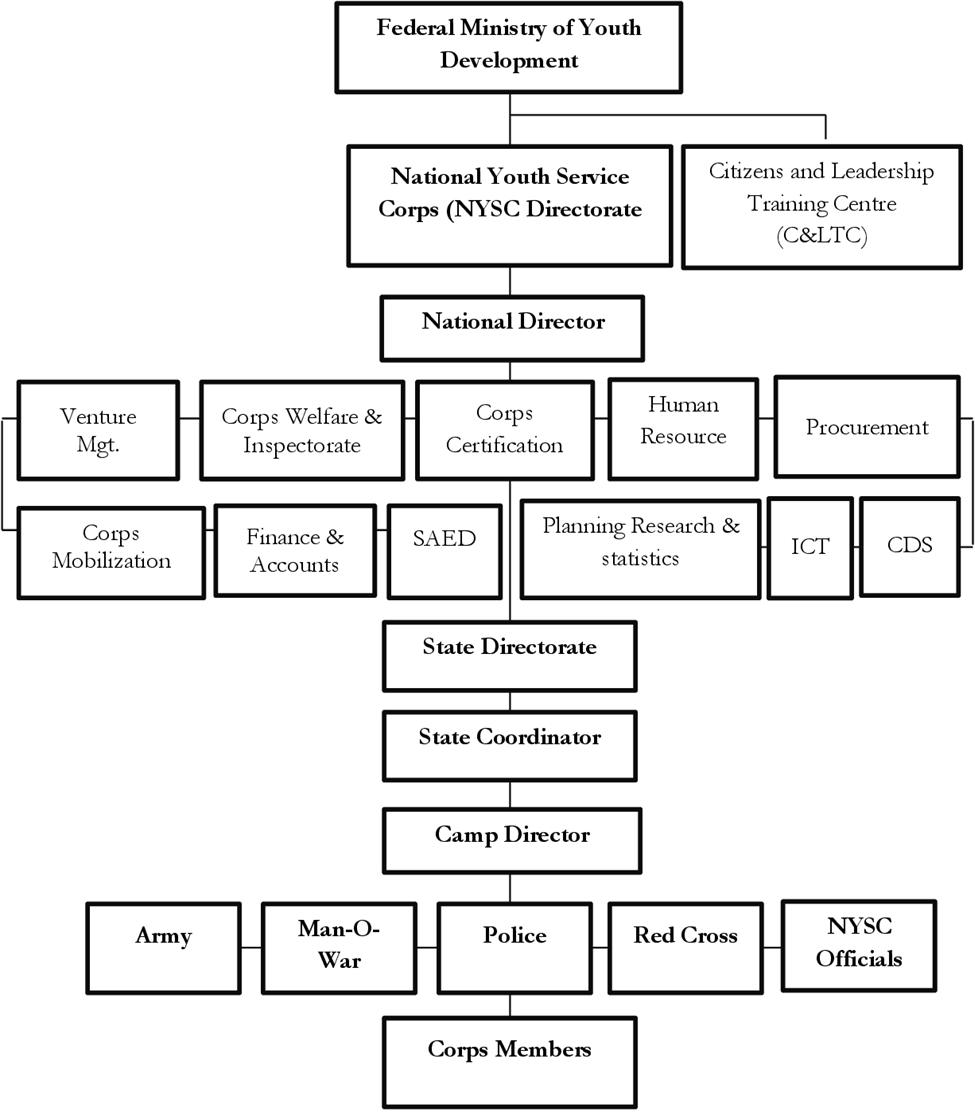
\includegraphics[scale = 0.4]{image2.png}
    \caption{\textit{Organogram of NYSC}}
    \label{fig:my_label}
\end{figure}

\section{Organogram of Drug Free CDS Executives}
\begin{figure}[H]
    \centering
    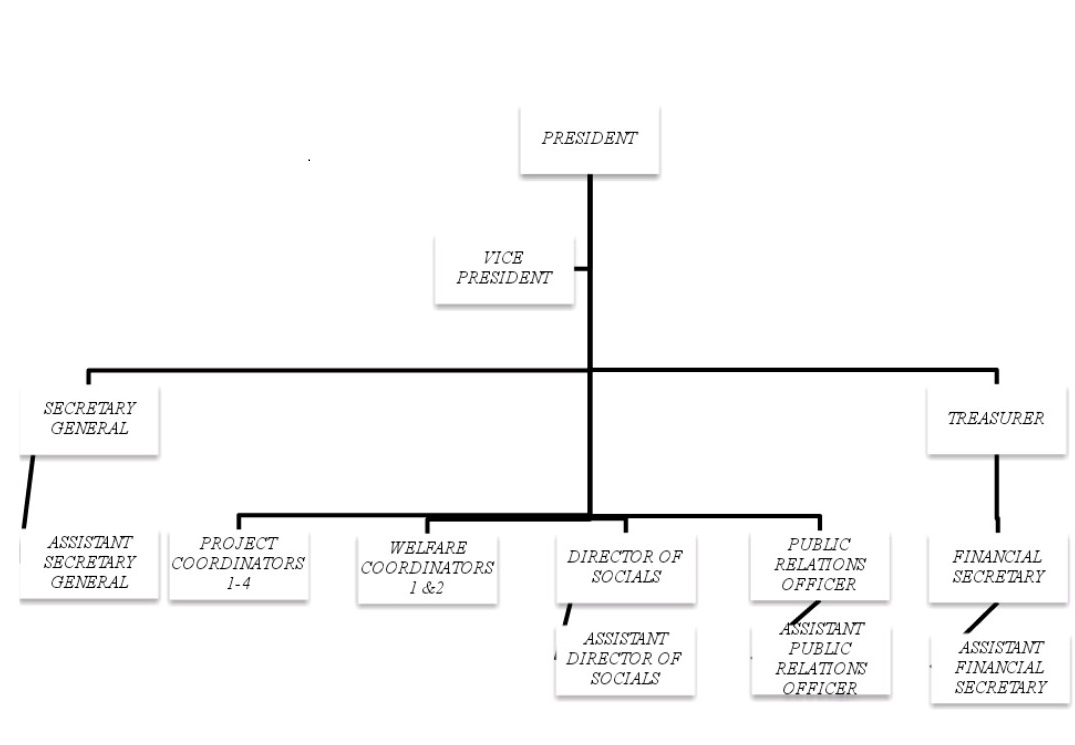
\includegraphics[scale = 0.4]{organogram.jpg}
    \caption{\textit{Organogram of Drug Free Club}}
    \label{fig:my_label}
\end{figure}

\section{NYSC Drug Free Club and Its Affiliate Organizations}
It is an established fact that through the NYSC Drug- Free Club; the National Youth Scheme has continued to work in collaboration with the National Drug Law Enforcement Agency (NDLEA), in order to ensure a drug free society.

The collaboration with NYSC is evidently part of the NDLEA’s efforts at tackling drug abuse among Nigerian Youths as the NYSC scheme has been helping the NDLEA in various schools and the streets in the campaign against drug abuse by educating the students and members of the general public on the dangers and consequences of drug abuse.
\\
\section{Drug Free Club Executives And Their Responsibilities}
\begin{enumerate}
    \item PRESIDENT
        \begin{itemize}
    \item 
    To set and monitor the goals of a particular administration.
    
    \item 
    To preside over meetings.
    
    \item 
    Appointing task officers to micromanage tasks.

    \item 
    To monitor other officials and ensure their duties are discharged efficiently.
    
    \item 
    To submit club attendance to the Corp Liaison Officer (C.L.O) for monthly clearance.
    
    \item 
    To lead the club.
\end{itemize}

    \item VICE PRESIDENT
        \begin{itemize}
    \item 
    Preside over the club in the absence of the president.

    \item 
    To assist in the running and overseeing of the club.
    
    \item 
    To assist executive members where necessary in discharging their duties.
\end{itemize}
    \item GENERAL SECRETARY
        \begin{itemize}
    \item 
    Planning meetings with the president.
    
    \item 
    Preparing meeting agendas.
    
    \item 
    Taking meeting minutes.

    \item 
    Circulating/ reading of last minutes before new meetings.
    
    \item 
    Keeping records of club activities.
    
    \item 
    Taking CDS meeting attendance.
\end{itemize}

    \item ASSISTANT GENERAL SECRETARY
        \begin{itemize}
    \item 
    Assisting the general secretary in his/her aforementioned duties.
    
    \item 
    To act as general secretary in the absence of the general secretary.
\end{itemize}

    \item FINANCIAL SECRETARY
        \begin{itemize}
    \item 
    To receive and document all fund transactions of the club including club dues, contributions and fines.
    
    \item 
    To handle the spending and refunds of finances within the club.
    
    \item 
    Deposit the funds of the club in the clubs account. In the event there is none, the treasurer or financial secretary’s account may be used.

    \item 
    To prepare detailed reports on the net income and expenditure of the club.

\end{itemize}

    \item ASSISTANT FINANCIAL SECRETARY
        \begin{itemize}
    \item 
    To assist the financial secretary in discharging his or her duties.
    
    \item 
    To act in place of the financial secretary in the event of absence.

\end{itemize}

    \item TREASURER
        \begin{itemize}
    \item 
    To oversee and ensure all financial systems are in place.
    
    \item 
    To oversee club budgets.
    
    \item 
    With the financial secretary, manage the clubs funding.

\end{itemize}

    \item DIRECTOR OF SOCIALS
        \begin{itemize}
    \item 
    To coordinate all social activities of the club including outings, sporting events, hangouts, etc.
    
    \item 
    To teach new members the club anthem as well as official greetings.

\end{itemize}

    \item ASSISTANT DIRECTOR OF SOCIALS
        \begin{itemize}
    \item 
    To assist the director of socials in their duties.
    
    \item 
    To act as the director of socials in the absence of the director of socials.

\end{itemize}

    \item WELFARE COORDINATOR 1 \& 2
        \begin{itemize}
    \item 
    To work with club executives to ensure a pleasant environment for the club members.
    
    \item 
    To handle club members complaints and present the to the executives for further actions.
    
    \item 
    To be in charge of refreshments during meetings.

\end{itemize}

    \item PUBLIC RELATIONS OFFICER
        \begin{itemize}
    \item 
    To communicate with the general public on behalf of the club e.g. via letters and announcements.
    
    \item 
    To anchor CDS meetings.
    
    \item 
    To pass information from the club executives to the club members.

\end{itemize}

    \item PROJECT COORDINATORS 1, 2, 3 \& 4
        \begin{itemize}
    \item 
    To handle and oversee ongoing club projects.
    
    \item 
    To take ideas from club members concerning club projects and present them to executives for further action.
    
\end{itemize}


\end{enumerate}

\chapter{Constitution}
\section{SECTION 1: PREAMBLE}
This Constitution is the Combination of law(s) put together the representation of the populace on the interest of every Drug Free CDS members. This constitution is Supreme and its provision shall be/have binding force in all authorities & persons of the Drug Free CDS If any other laws are inconsistent with the provision of this constitution except the fundamental NYSC Laws, this Constitution shall prevail and any other laws shall to the extent of the inconsistency be void.

However, this constitution is subject to future and further Amendment by the following factors; 
\begin{enumerate}
    \item Election Manifesto
    
    \item Doctrine of mandate
     
    \item Public CDS opinion and doctrine of consultation with vested interest if need be.
\end{enumerate}


\subsection{SECTION 1B: Purpose of this Constitution}
\begin{itemize}
    \item To Create Law and order; because where there is law, there is Remedy. 
    
    \item To unite ever member of the Drug free CDS.
     
    \item To Produce responsible membership within the CDS is to fully dispense equitable justice, freedom and equality of Law & Order.
    
    \item To enhance dynamic, healthy, resourceful, articulated and unsegmented CDS Group. 
\end{itemize}


\subsection{SECTION 1C: Executive Members}
The Drug Free CDS shall have the following Executive Portfolios;
\begin{enumerate}
    \item The President 
    \item Vice President
    \item General Secretary
    \item Assistant General Secretary
    \item The project Coordinator 1, 2, 3, 4
    \item Financial secretary 
    \item Assistant Financial secretary.
    \item The Treasurer
    \item The Director of welfare
    \item Assistant Director of welfare
    \item The Director of social 
    \item Assistant Director of social 
    \item The Public Relation officer
    \item Assistant Public Relation Officer
\end{enumerate}

\section{SECTION 2: Executive Electoral nomination rules}
% use \Alph*. option to enable A. labeling of itemized option.
\begin{enumerate}[label = \Alph*. ] 
    \item Any Person Contesting for any position in the Drug Free CDS must have at least 3 month left before the termination of his & her services year.
    
    \item Every gender is permitted and qualify for any post in the Drug Free CDS.
    
    \item Every electoral activities shall be carry out in an CDS meeting where only members of Drug Free CDS shall participates in the electoral process.
    
    \item Nominations of any person to an Executive post or to carry out any task shall equally be done in CDS meeting. However final decision shall be communicated back to the general member by the Public Relation officer or the General secretary after some qualitative examinations & checks by the Executives. 
    
    \item Executives shall be able to Nominate in need arises. Then, The President shall appoint a suitable candidate.
    
    \item Suitable Candidates for the nomination or electoral appointment should have consistent attendance for prior to nomination.
    
    \item Suitable Candidates for the nomination or electoral appointment must diligently pay their dues prior to nomination or candidacy.
\end{enumerate}

\section{SECTION 3: Absenteeism}
\begin{enumerate}[label = \Alph*. ] 
    \item Any member who to not meet up to 2/3 of CDS meeting shall not be covered by attendance to do clearance.
    
    \item Any member who do not present him/her self in the CDS meeting in a period of (4 weeks) a month shall be  assume to have left the CDS.
    
    \item Any Executive is found absent for Consecutive 3 CDS meeting  without due permission of notable reason and evidence will be deemed to have voluntarily withdrawn his or herself from the position.
\end{enumerate}

\section{SECTION 3: CDS Attendance}
\begin{enumerate}[label = \Alph*. ] 
    \item Any person who was absent without prior notification worthy and provable to the President or the General secretary shall not be allows into the attendance for the week.
    
    \item Any person  found late to CDS meetings Shall be liable to a fine decided by the Executives. 
    
    \item Any person found unlawfully signing attendance on behalf of an absentee shall be punishable as decided.
    
    \item All CDS benefits such as participant certificate amongst other shall be attendance based. 
    
    \item It shall be Compulsory for every CDS member to attend Sensitization outing and any one found otherwise shall be punishable Except If It is a delegated Sensitization.
\end{enumerate}

\section{SECTION 5: Payment of dues}
\begin{enumerate}[label = \Alph*. ] 
    \item All Drug Free CDS dues shall be paid to the financial secretary Except If directed otherwise and such direction must be declared in public.
    
    \item All Drug Free CDS members shall pay his or her CDS dues within the Speculated time frame and if done otherwise shall pay double.
    
    \item Any Drug Free CDS executive who refuses to pay the monthly dues for two consecutive months would be remove from his/her office.
\end{enumerate}

\chapter{Drug Free CDS Meeting}

Drug Free CDS meeting starts by 9:00am prompt and ends 10:30am
*The Drug Free CDS holds at the NDLEA office along Ijoko Road, Sango Otta Ogun State or holds at the Secretariat (Ado-Otta) and this is done every Thursday of every month.

\section{Types of meetings}
\begin{enumerate}
    \item Social Meetings 
    
    \item Sensitization Meeting
    
    \item General CDS meeting
\end{enumerate}

\subsection{The social meeting}
This is a meeting where we corp members of drug free CDS gather in our venue (NDLEA/SECRETARIAT) to have all sorts of games examples we have charades, using words for sentence and all..

\subsection{The sensitization meeting}
This is a meeting whereby our goal as a corp member is to stimulate the transition from stakeholder awareness to relevant information based on the possible guidelines for change needed to facilitate environment conducive to healthy lifestyles and this is where we get to go to different organizations such as companies, schools, bus-stop, garage, and so on.

\subsection{Agenda of Meetings}
\begin{itemize}
    \item Meaning of sensitization 
    
    \item Examples of sensitization  
    
    \item Goal/Aims of sensitization 
    
    \item opening prayer 
    
    \item Introduction of new members
    
    \item Introduction/Opening Remarks 
    
    \item Song of drug free 
    
    \item Deliberation on project work
    
    \item Overview of plans for the tenure
    
    \item Closing Prayer
\end{itemize}

\section{Club Culture}
The Drug Free Club has specific practices done during its meeting to signify respect and unity among its members and associated officers. These practices include a song, a welcome protocol and an official greeting.

\subsection{Club Song}
\textit{Oya Drug Free, Ja Lo Oo\\
Away Aye\\
\\
To the place where we wan go ah\\
Away Aye\\
\\
She we go dey spend our lives, oo\\
Away Aye\\
\\
Oya Drug Free, Ja Lo Oo\\
Oo, Ja Lo Oh\\
}


\subsection{Welcome Protocol}
The President\\
The Vice President\\
The General Secretary\\
The Treasurer\\
Executive members\\
Friends and guests in our midst\\
My fellow members\\
\\
I am Drug Free Club Member ...........................................................................................................,\\ graduate of ..................................................................... at the university or polytechnic or college of education ...........................................................................................\\ My Place of Primary Assignment is ........................................................................

\subsection{Official Greeting}
\textit{\textbf{On encountering an NDLEA officer,}}\\
\\
CALLER: Drug Free Members present salute\\
\\
MEMBER: **Members stand with hand at thier side, chest forward and legs together** All together chant, Morning Sir.

\textbf{**Sitting Member stretch their arms forward, chest out and chant the greeting.**}

\chapter{Drug Abuse}
\section{Drug Use Disorder, Abuse, Substance Abuse and Addiction}

Formerly separately called substance or \textbf{drug abuse and addiction}, drug use disorder, also called substance use or chemical use disorder, is an illness characterized by a destructive pattern of using a substance that leads to significant problems or distress, including tolerance to or withdrawal from the substance, as well as other problems that use of the substance can cause for the sufferer, either socially or in terms of their work or school performance.

\textbf{Drug abuse} is a situation when drug is taken more than it is prescribed. It could be seen as the use of illicit drugs, or the abuse of prescription or over-the-counter drugs. It could further be defined as the deliberate use of chemical substances for reasons other than intended medical purposes and which results in  physical,  mental, emotional or social impairment of the user. The abuse of legal drugs  can happen when people use the drugs in a manner other than directed by the manufacturer or purpose that are not legitimate. According  to the  National Agency  for Food and Drug Administration and Control (NAFDAC), \textbf{drug abuse} is seen as excessive and persistent self-administration of a drug without regard to  the medically or culturally accepted patterns. 

Similarly,  the  World  Book Encyclopedia views \textbf{drug abuse} as the non-medical use of a drug  that interferes with a healthy and productive  life. According to World Health Organization11, \textbf{substance abuse} is the harmful or hazardous use of psychoactive substances, including alcohol and illicit drugs. World Health Organization (WHO) also reports that it is estimated that about 76.3 million people struggle with alcohol use disorders contributing to 1.8 million deaths per year. \textbf{Drug addiction} is the excessive,  mal-adaptive, or obsessive use of   drugs   for non-medicinal purposes. It is characterized by a compulsion to take drugs on a steady basis in order to experience its mental effects. Drug addiction leads to habitual dependence on drugs which gives rise  to  mental, emotional, biological or physical, social and economic instability.

\section{Types of Drugs}
There are many types of drugs available, but we would elucidate the most commonly abuse categories in Nigeria.

\begin{enumerate}
    \item Stimulants: These are substances that directly act and stimulate the central nervous system. Users at the initial stage experience pleasant effects such as energy increase. The major sources of these come from caffeine substances.
    
    \item Hallucinogens: These are drugs that alter the sensory processing unit in the brain. Thus, producing distorted perception, feeling  of anxiety and euphoria, sadness and inner joy, they normally come from marijuana, LSD etc.
    
    \item Narcotics: These drugs relive pains, induce sleeping and they are addictive. They are found in heroin, codeine, opium etc.
    
    \item Sedatives: These drugs are among the most widely used and abused. This is largely due to the belief  that they relieve stress and anxiety, and some of them  induce  sleep, ease tension, cause relaxation or help users to forget their problems. They are sourced from Valium, alcohol, promethazine, chloroform.
    
    \item Tranquilizers: They are believed to produce calmness without bringing drowsiness; they are chiefly derived from Librium, Valium, and others. 
    
    \item Miscellaneous: This is a group of volatile solvents or inhalants that provide euphoria, emotional dis-inhibition and perpetual distortion of thought to the user. The main  sources are glues, spot removers, tube repair, perfumes, chemicals, etc. 
\end{enumerate}


\subsection{Examples of Commonly Abused Drugs}
\begin{enumerate}
    \item Alcohol: Although legal, alcohol is a toxic substance, especially for a developing fetus when a mother consumes this drug during pregnancy. One of the most common addictions, alcoholism can have devastating effects on the alcoholic individual's physical well-being, as well as his or her ability to function inter-personally and at work.
    
    \item Amphetamines: This group of drugs comes in many forms, from prescription medications like methylphenidate (for example, Ritalin, Concerta, Focalin) and dextroamphetamine and amphetamine (Adderall) to illegally manufactured drugs like methamphetamine ("crystal meth"). Overdose of any of these substances can result in seizures and death.
    
    \item Anabolic steroids: A group of substances that are most often abused by bodybuilders and other athletes, this group of drugs can lead to devastating emotional symptoms like aggression and paranoia, as well as severe long-term physical effects like infertility and organ failure.
    
    \item Caffeine: While many people consume coffee, tea, and soda, when consumed in excess, this substance can be habit-forming and produce palpitations, insomnia, tremors, irritability, and significant anxiety.
    
    \item Cannabis: More usually called marijuana, the scientific name for cannabis is tetrahydrocannabinol (THC). Marijuana is the most commonly used illicit drug, with nearly 14 million people 12 years or older reporting having used this drug in the past year. In addition to the negative effects, the drug itself can produce (for example, infertility, difficulties with sexual performance, paranoia, lack of motivation), the fact that it is commonly mixed (cut) with other substances so drug dealers can make more money selling the diluted substance or expose the user to more addictive drugs exposes the marijuana user to the dangers associated with those added substances. People commonly cut marijuana with ingredients that include baby powder, oregano, embalming fluid, phencyclidine (PCP), opiates, and cocaine.
    
    \item Cathinones (bath salts): Chemically unrelated to bath salts that people use to bathe, cathinone are chemically similar to stimulant drugs, like amphetamines, cocaine, and Ecstasy (MDMA). In addition to bath salts, other street names for cathinone include "plant food," "jewelry cleaner," or "phone screen cleaner."

    \item Cocaine: A drug that tends to stimulate the nervous system, people can snort cocaine in powder form, smoke it when in the form of rocks ("crack" cocaine), or inject it when made into a liquid.
    
    \item Ecstasy: Also called MDMA to denote its chemical composition (methylenedioxymethamphetamine), this drug tends to create a sense of euphoria and an expansive love or desire to nurture others. In overdose, it can increase body temperature to the point of causing death.
    
    \item  Hallucinogens: Examples include LSD and mescaline, as well as so-called naturally occurring hallucinogens like certain mushrooms. These drugs can be dangerous in their ability to alter the perceptions of the user. For example, a person who is intoxicated ("high" on) with a hallucinogen may perceive danger where there is none and think that situations that are truly dangerous are not. Those misperceptions can result in dangerous behaviors (like jumping out of a window because the person thinks they have wings and can fly).
    
    \item Inhalants: One of the most commonly abused groups of substances due to its easy accessibility, inhalants are usually in household cleaners, like ammonia, bleach, and other substances that emit fumes. Brain damage, to the point of death, can result from using an inhalant even just once or over the course of time, depending on the individual.
    
    \item Nicotine: The addictive substance found in cigarettes, nicotine is actually one of the most addictive substances that exist. In fact, people often compare nicotine addiction to the intense addictiveness associated with opiates like heroin.
    
    \item Opiates: People also call this group narcotics or opioids and include drugs like heroin, codeine, hydrocodone, morphine, methadone, Vicodin, OxyContin, Percocet, and Percodan. This group of substances sharply decreases the functioning of the nervous system. The lethality of opioids is often the result of the abuser having to use increasingly higher amounts to achieve the same level of intoxication, ultimately to the point that the dose needed to get high is the same as the dose that is lethal by overdose for that individual by halting the person's breathing (respiratory arrest).
    
    \item Phencyclidine: Commonly called PCP, this drug can cause the user to feel highly suspicious, become very aggressive, and have an exceptional amount of physical strength. This can make the person quite dangerous to others.
    Sedative, hypnotic, or antianxiety drugs: The second most commonly used group of illicit drugs, these substances quiet or depress the nervous system. They can therefore cause death by stopping the breathing (respiratory arrest) of the individual who either uses these drugs in overdose or who mixes one or more of these drugs with another nervous system depressant (like alcohol, another sedative drug, or an opiate
\end{enumerate}

\section{Effects of Drug Abuse}
The effects of drug abuse among Nigerian youths are numerous. Commonly identified the following as
the negative effects of drug abuse on the body chemistry of the users:
\begin{itemize}
    \item Alcohol-related problems include: 
    \begin{itemize}
        \item Physical problems e.g. liver cirrhosis, pancreatic, peptic ulcer, tuberculosis, hypertension,neurological disorder.
        
        \item Mental  retardation   for   the   fetus   in   the   womb,   growth,   deficiency,   delayed motor development.
        
        \item Craniofacial abnormalities, limbs abnormalities and cardiac deficits.
        
        \item Psychiatric e.g. pathological drunkenness, suicidal behavior.
        
        \item Socially-broken homes, increased crime rate, sexual offences, homicide and sexually transmitted diseases.
    \end{itemize}
    
    \item Tobacco-related problems include: Causes stimulation of heart and narrowing of blood  vessels,  producing hypertension, headache, loss of appetite, nausea and delayed growth of the fetus. It also aggravates  or causes sinusitis, bronchitis, cancer, strokes and heart attack.
    \item Stimulants:   Lethargy,   irritability,   exaggerated   self-confidence,   damage   nose linings, sleeplessness, and psychiatric complications.
    
    \item Inhalants: Causes anemia, damage kidney and stomach bleeding.
    
    \item Narcotics:  Causes poor perception, constipation, cough,  suppression, vomiting, drowsiness and sleep, unconsciousness and death.
    
    \item Other generally-related issues include:
    \begin{itemize}
        \item Diseases: Spread diseases such as HIV/AIDS and Hepatitis C through sharing needles, or having unprotected sex.
        
        \item Crime: Drug addicts and abusers are likely to engage in Drug possession/use, Drug trafficking, Robbery, Prostitution and other sex crimes, and Terrorism (political gangsters).
        
        \item Craniofacial abnormalities, limbs abnormalities and cardiac deficits.
        
        \item Psychiatric e.g. pathological drunkenness, suicidal behavior.
        
        \item Socially-broken homes, increased crime rate, sexual offences, homicide and sexually transmitted diseases.
    \end{itemize}
    
\end{itemize}

\section{Causes of drug addiction}
Drug addiction refers to the compulsive and repeated use of increasing amounts of drugs with the appearance of withdrawal symptoms when drug use ceases. While the specific causes of drug addiction are not known, genetic, psychological and environmental factors are thought to play a significant role. Rather than a single cause of drug addiction, it is likely multiple factors lead to drug addiction in any given person.

Some drug addict also identify drug use and ignorance as a cause of drug addiction. Often, if a person is dealing with pain-management issues, the drug they receive, like oxycodone, can be very addictive. The ignorance of the drug's addiction potential, along with the physical pain of the condition, becomes a cause of drug addiction.

The field of addiction draws upon a variety of  disciplines. Psychology, medicine, chemistry, psychiatry, sociology, biology and physiology have all helped shape current understandings of addictive behavior. The major emphasis of the theories is that people have their individual reasons for depending on one type of drug or the other.

\subsection{Biological Causes of Drug Addiction}
This theory  maintains that  drug abuse is determined  by the individual’s biological or genetic factors which make  such individual vulnerable to drug addiction. This is a composition of three main theories of causes of drug abuse.

Other related theories include: 
\begin{enumerate}
    \item \textbf{Personality Theory of Drug Abuse}: The main emphasis of the theory is that there is certain a trait or characteristics in the individual that yield to abuse of drugs. Such personality characteristics are inability to delay gratification, low tolerance for frustration, poor impulse control; high emotional dependence on other people, poor coping ability and low self-esteem. Individuals with these personality characteristics find it difficult to abstain from drug abuse. 
    
    \item \textbf{Learning Theory of Drug Abuse}: It maintains that dependence or abuse of drugs occur as a result of learning. The learning could be by means of conditioning, instrumental learning or social learning.
\end{enumerate}

\subsection{Psychological Causes of Drug Addiction}
While biological causes of drug addiction have been suggested, many people still believe psychological factors comprise the bulk of what causes drug addiction. Some of the psychological causes of drug addiction appear to stem from trauma, often when the drug addict is young. Sexual or physical abuse, neglect, or chaos in the home can all lead to psychological stress, which people attempt to "self-medicate" (decrease the stress's pain through drug use). This self-medication becomes a cause of drug addiction.

Psychological causes of drug addiction include:
\begin{itemize}
    \item 
    A mental illness such as depression
    
    \item
    Inability to connect with others, lack of friends
    
    \item
    Poor performance at work or school

    \item
    Poor stress coping skills
\end{itemize}


\subsection{Environmental Causes of Drug Addiction}
A person's environment can be part of what causes drug addiction. Drug addiction is more common in environments where drug abuse is seen or where it's seen as permissible. Children who grow up in homes with drug addicts often become drug addicts themselves.

Because most drug use starts in adolescence, Those with inattentive, abusive or neglectful parents are more prone to drug abuse. One cause of drug addiction can be the combination of drug and the lack of parental oversight.
Other environmental factors that can be causes of drug abuse include:
\begin{enumerate}
    \item 
    Participation in a sport where performance-enhancing drugs are encouraged
    
    \item
    A peer group that uses or promotes drug use
    
    \item
    People of lower socioeconomic status are at greater risk of drug addiction

    \item
    Gender and ethnicity contribute to addiction of some drugs
\end{enumerate}

\subsection{Genetic Causes of Drug Addiction}
Drug addiction tends to run in families, indicating genetics may have a role in causing drug addiction. In fact, in studies of twins it appears half of someone's risk of becoming addicted to drugs is genetic  (tell us more or avoid it altogether). Genetic causes of drug addiction appear to involve multiple gene sequences and science has not yet been able to pinpoint all the genes involved. However, it is known some genes, like those involved in brain receptors of nicotine, contribute to the cause of drug addiction. \footnote{Drug Abuse And Its Effects In Nigeria | Akonbede Udama - Academia.edu – section 2, 3 and 4.}

\section{Measures to Curb Drug Abuse}
An important method of curbing drug abuse and eventual addiction in the society is teaching individuals to signs and symptoms. Identifying these signs especially in youths and young adults would go a long way to ensure proper treatment and care are administered.  


\subsection{Warning Signs of Drug Abuse}
Drug abusers often try to conceal their symptoms and downplay their problem. If you’re worried that a friend or loved one might be abusing drugs, look for the following warning signs:

\begin{itemize}
    \item Physical warning signs 
    \begin{itemize}
    \item Bloodshot eyes, pupils larger or smaller than usual
    \item Changes in appetite or sleep patterns
    \item Sudden weight loss or weight gain
    \item Neglecting one’s appearance
    \item Deterioration of physical appearance, personal grooming habits
    \item Unusual smells on breath, body, or clothing
    \item Tremors, slurred speech, or impaired coordination
    \end{itemize}

    \item Behavioral warning signs
    \begin{itemize}
    \item Drop in attendance and performance at work or school
    \item Unexplained financial problems; borrowing or stealing
    \item Engaging in secretive or suspicious behaviors
    \item Sudden change in friends, favorite hangouts, and hobbies
    \item Frequently getting into trouble (fights, accidents, illegal activities)
    \end{itemize}
    
    \item Psychological warning signs 
    \begin{itemize}
    \item Unexplained change in personality or attitude
    \item Sudden mood swings, irritability, or angry outbursts
    \item Periods of unusual hyperactivity, agitation, or giddiness
    \item Lack of motivation; appears lethargic or “spaced out”
    \item Appears fearful, anxious, or paranoid
    \end{itemize}

\end{itemize}


\subsection{Common Signs and Symptoms Drugs Addiction }
\begin{itemize}
    \item Problems at work or school, including poor performance,
    \item lateness or absenteeism and social dysfunction.
    \item Loss of energy or motivation
    \item Neglecting one’s appearance
    \item Spending excessive amounts of money on the substance
    \item Stealing to get the drug
    \item Performing risky behaviors while intoxicated
    \item Compulsively taking the drug or being unable to stop taking it.
\end{itemize}

\subsection{Treatments for drug addiction}
There are many options that have been successful in treating drug addiction, including:
\begin{itemize}
\item Behavioral counseling
\item Medication
\item Medical devices and applications used to treat withdrawal symptoms  or deliver skills training
\item Evaluation and treatment for co-occurring mental health issues such as depression and anxiety
\item Long-term follow-up to prevent relapse
\end{itemize}

A range of care with a tailored treatment program and follow-up options can be crucial to success. Treatment should include both medical and mental health services as needed. Follow-up care may include community or family-based recovery support systems. Please include agencies like the NDLEA and others Non Governmental Organizations with trained professions for help with treatments or overdose issues.


\end{document}